\chapter{Introduction} \label{chap:intro}
Scientific Computing (SC) is at the intersection of computer science, 
mathematics, and science. SC analyses and simulates mathematical methods of 
complex scientific and engineering problems by using computing techniques and 
tools. To improve understandability, maintainability, and reproducibility, 
writing documentation should be part of the process of developing scientific 
software. The role of documentation is to help people better understand the 
software and to ``communicate information to its audience and instill knowledge 
of the system it describes" \cite{forward2002software}. The significance of 
software documentation has been presented in many papers by previous 
researchers. High-quality documentation serves as the foundation for effective 
communication within software development teams, while also contributing to the 
overall excellence of the software product \cite{parnas2011precise, 
chomal2014significance, kipyegen2013importance}. Additionally, Smith et al. 
\cite{SmithandKoothoor2016, SmithandYu2007} shows that developing SC software 
in a document-driven methodology potentially improves the quality of the 
software. 

Jupyter Notebook is a popular approach for documenting SC software, providing a 
system for creating and sharing data science and scientific computing 
documentation and code. This nonprofit, open-source application was born in 
2014. Jupyter Notebook provides interactive computing across multiple 
programming languages, such as Python, Javascript, Matlab, and R. A Jupyter 
Notebook integrates text, live code, equations, computational outputs, 
visualizations, and multimedia resources, including images and videos. Jupyter 
Notebook is one of the most widely used interactive systems among scientists. 
Its popularity has grown from 200,000 to 2.5 million public Jupyter Notebooks 
on GitHub in three years from 2015 to 2018 \cite{Jeffrey2018}. It is used in a 
variety of areas and ways because of its flexibility and added values. For 
example, Notebooks can be used as an educational tool in engineering courses, 
enhancing teaching and learning efficiency \cite{cardoso2019using, zhao2019use}.

Even though the importance of documentation is widely recognized, it is often 
missing or poorly realized in SC software because: i) scientists are not aware 
of the why, how, and what of documentation \cite{hermann2022documenting, 
chang2022understanding}; ii) it is time-consuming to produce 
\cite{sanders2008dealing}; iii) scientists generally believe that writing 
documentation demands more work and effort than they would likely yield in 
terms of the benefits of it \cite{smith2016advantages}.

Jupyter Notebook simplifies the process of maintaining SC documentation by 
enabling explanatory text and code to be combined in a single document. 
Furthermore, it provides easy sharing of notebooks on platforms like GitHub and 
exportation to different formats, such as PDF. However, there are also some 
downsides to employing it. While Jupyter Notebook streamlines documenting code, 
it can be more challenging to maintain and refactor the code itself, especially 
when dealing with large datasets or complex code. Debugging and refactoring 
code across multiple segments, for instance, can be time-consuming and 
difficult to test. Poor coding practices may lead to poor quality and 
reproducibility of Jupyter Notebooks \cite{pimentel2021understanding, 
wang2020better}.

We are trying to increase the efficiency of documentation development by 
adopting generative programming. Generative programming is a technique that 
allows programmers to write the code or document at a higher abstraction level, 
and the generator produces the desired outputs. Drasil is an application of 
generative programming, and it is the framework we use to conduct this 
research. Drasil saves us more time in the documentation development process by 
letting us encode each piece of information of our scientific problems once and 
generating the document automatically.

In this chapter, we will provide an introduction to Drasil and Jupyter 
Notebook, including their usage and benefits. Following this, we will delve 
into the problems that our paper aimes to address.

\section{Background}
Chapter~\ref{chap:intro_drasil} gives a general introduction to Drasil, and
Chapter~\ref{chap:intro_notebook} discusses the features and benefits of 
Jupyter Notebook.

\subsection{Drasil} \label{chap:intro_drasil}
Drasil is a framework that can generate software artifacts, including Software 
Requirement Specifications (SRS), code (C++, C\#, Java, and Python), README, 
and Makefile, from a stable knowledge base. The goals of Drasil are reducing 
knowledge duplication and improving traceability \cite{drasil}. Drasil captures 
the knowledge through our hand-made case studies. We currently have 10 case 
studies that cover different physics problems, such as Projectile motion and 
double Pendulum simulation. Recipes for scientific problems are encoded in 
Drasil, which then generates code and documentation for us. Each piece of 
information only needs to be provided to Drasil once, and that information can 
be used wherever it is needed. By defining and storing common concepts in a 
central repository and case-specific concepts in their own packages, Drasil 
enables the reuse of information across different engineering domains and 
applications. This feature significantly reduces the time and effort required 
for software development and documentation, while also improving the 
consistency and accuracy of the information being used. Later in the chapters, 
we will discuss the details of how information is encoded and how knowledge is 
reused in Drasil.

The SRS is built using a template for designing and documenting scientific 
computing software requirements as created by Smith et al \cite{smith2005new}. 
Drasil is currently capable of generating an SRS in the document languages HTML 
and LaTeX. We are looking to extend the capability of Drasil by generating 
Jupyter Notebooks in Drasil.

\subsection{Jupyter Notebook} \label{chap:intro_notebook}
Jupyter Notebook is an interactive open-source web application for creating and 
sharing computational science documentation that contains text, executable 
code, mathematical equations, graphics, and visualizations.

\subsubsection{Structure of a notebook document}
A Jupyter Notebook has two components: front-end ``cells" and back-end 
``kernels". The notebook consists of a series of cells, which can be code 
cells, Markdown cells, or raw cells. A cell is a multiline text input field. 
The notebook follows a sequential flow, where users entering a piece of 
information, either in the form of text or programming code, into the cells 
from the web page interface. This information is then sent to the back-end 
kernels for execution, and the results are return to the user 
\cite{notebookdoc}. Figure~\ref{fig:running_code} shows an example of a
Jupyter Notebook \cite{jupyternotebookrep}.

\begin{figure}[h!]
	\caption{Example of a Jupyter Notebook}
	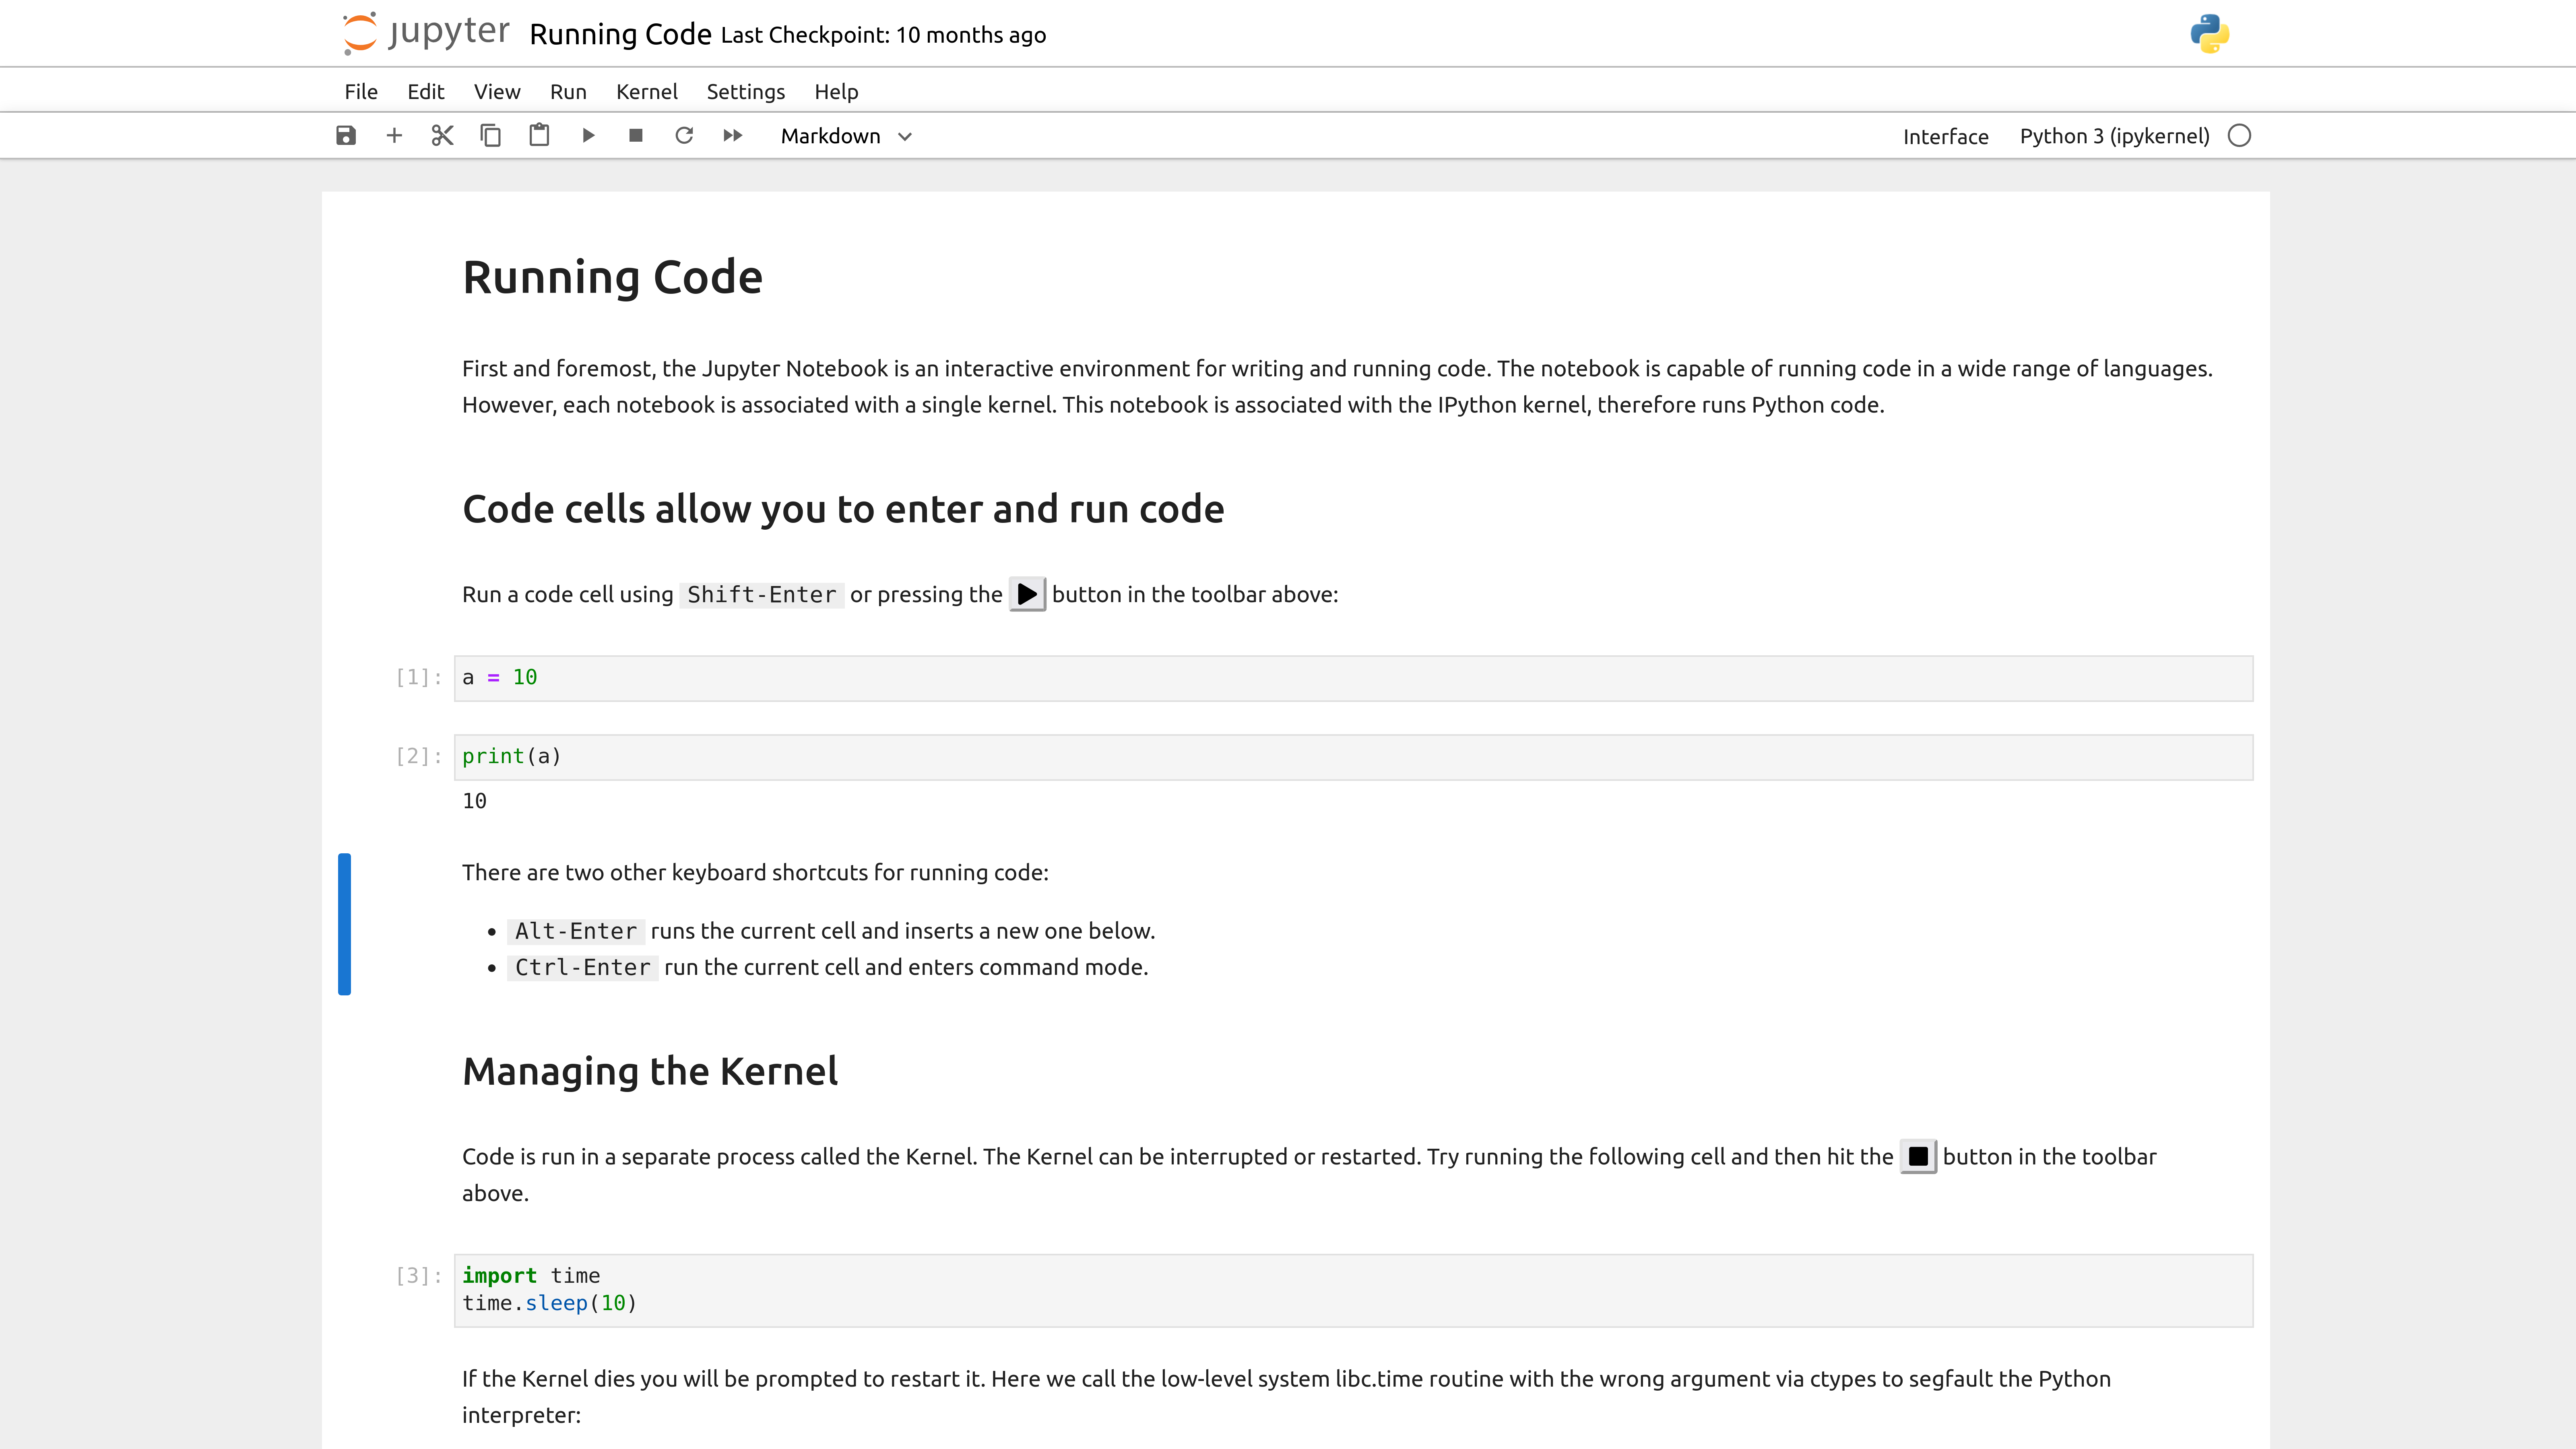
\includegraphics[width=1\textwidth]{figures/running_code.png}
	\label{fig:running_code}
\end{figure}

\subsubsection{The Value of Jupyter Notebooks}
There are several advantages of Jupyter Notebook: sharable, all-in-one, and 
live code. First of all, the notebook is easy to share because it can be 
converted into other formats such as HTML, Markdown, and PDF. This is 
advantageuous because it allows someone working on a notebook to share it with 
others without requesting that they install any additional software and making 
it easier to collaborate on the projects. Secondly, Jupyter Notebooks combine 
all aspects of data in one single document, making the document easy to 
visualize, maintain and modify. In addition, they provide an environment of 
live code and computational equations. Usually, when programmers are running 
code on some other IDEs, they have to write the entire program before executing 
it. However, the notebook allows programmers to execute a specific portion of 
the code without running the whole program. The ability to run a snippet of 
code and integrate with text highlight the usability of the notebook. Previous 
research has demonstrated that Jupyter Notebooks can significantly contribute 
to reproducibility, reusability, and more effective computational workflows in 
science \cite{beg2021using}.

\section{Problem Statement}
Since both Jupyter Notebook and Drasil focus on creating and generating 
scientific computing documentation, we are interested in extending the values 
of Jupyter Notebook to Drasil and the kind of knowledge we can manipulate. 
Following are the three main problems we are trying to solve with Drasil in 
this paper:

\begin{enumerate}
	\item Generate Jupyter Notebooks. To acheive this, we will have 
	to generate documents in notebook format. Jupyter Notebook is a simple 
	JSON document with a .ipynb file extension. Notebook contents are either 
	code or Markdown. Therefore, non-code contents must be in Markdown format 
	with JSON layout. Drasil can currently write in HTML and LaTeX. We are 
	building a notebook printer in Drasil for generating documents that are 
	readable and writable in Jupyter Notebook.
	\item Develop the structure of lesson plans and generate them. As 
	mentioned, Jupyter Notebook is used as an educational tool for teaching 
	engineering courses. When it comes to teaching, lesson plans are often 
	brought up because they help teachers to organize the daily activities 
	in each class time. We are interested in teaching Drasil a ``textbook" 
	structure by starting with generating a simple physics lesson plan and 
	expanding Drasil's application. We aim to capture the elements of 
	textbook chapters, identify the family of lesson plans, and classify the 
	knowledge to build a general structure in Drasil, which will enable the 
	lesson plan to generalize to a variety of lessons.
	\item Generate notebooks that mix text and code. Jupyter Notebook is 
	an interactive application for creating documents that contain formattable 
	text and executable code. However, Drasil doesn't currently support 
	interactive recipes. There is no code in SRS documents, and text and code 
	are generated separately in Drasil. We are looking for the possibility of 
	generating a notebook document that incorporate both text and code, thereby 
	enhancing the capabilities of Drasil and its potential to solve more 
	scientific problems.
\end{enumerate}

\section{Thesis Outline}
Chapter~\ref{chap:nbprinter} covers the topic of how Drasil generates and 
prints documents using the Drasil printer, as well as the creation of the 
notebook printer for generating Jupyter Notebooks in Drasil. Moving on to 
Chapter~\ref{chap:lessonplan}, we discuss the structure of lesson plans, how we 
define the lesson plans language in Drasil, and how to generate them with the 
notebook printer. Chapter~\ref{chap:codeBlock} discusses various approaches for 
splitting the contents to mix different types of content, such as text and 
code, in Jupyter Notebooks with Drasil, as well as the implementation for 
generating code blocks. Lastly, Chapter~\ref{chap:conclusion} provides an 
overview of the future work and concludes the achievements of this work.